\section{Introduction}
% Introduction 
% <<<
The Stokes equations \eqref{unsteady_stokes}, which are solved for an incompressible Navier-Stokes flow,
assume the Reynolds number is $Re \ll 1$ and thus advective processes are neglible in comparison to viscous processes.
The nonlinear term of the Navier-Stokes equations are then neglected, resulting in a far more numerically tractable set of equations.
The goal here is to derive and implement a linear Stokes flow solver, which can then be used as a component of a Navier-Stokes solver,
described in the next chapter.
We will solve, in particular, the steady-state form \eqref{steady_stokes}.
Due to this simplification, the Steady stokes equations \eqref{steady_stokes}, repeated here:
\begin{align*}
    -\nu\Delta u = -\nabla p + \rho g, \quad \nabla\cdot u = 0,
\end{align*}
form a constrained linear equation. As we saw in section \ref{pressure_derivation}, the pressure term $p$ is a Lagrange multiplier introduced
with the constraint $\nabla\cdot u = 0$.

\subsection{The lid-driven cavity flow problem}
A standard test case in computational fluid dynamics is the \textit{lid-driven cavity flow} problem.
We let the domain be is $\Omega = [-1,1]^2$ and define a Dirichlet boundary condition:
\begin{equation}\label{lid_driven_boundary_condition}
    \left.u\right|_\Gamma = u_\Gamma(x,y) =
    \left\{\begin{array}{lr}
        \left(1, 0\right)^T &\text{if $y = 1$,}\\
        \left(0, 0\right)^T &\text{otherwise}.\\
        \end{array}\right.
\end{equation}
We will use a finite element method to solve the steady Stokes flow \eqref{steady_stokes} with this domain and boundary condition. A highly viscous incompressible
fluid under these conditions will form a single stable vortex.

\section{Attempting solution by an iterative pressure update}
% <<<
Since the steady Stokes equations are a linearly constrained vector Poisson equation,
it would be convenient to use a solution method which trivially extends our already-implemented Poisson solver.
One idea is to define a coupled system of equations replacing the constrained equation \eqref{steady_stokes}, resulting in an initial boundary value problem
in auxilliary parameter $\gamma$:
\begin{equation}
\begin{split}
    -\nu\Delta u &= -\nabla p_* + \rho g,\\
    \Part{p_*}{\gamma} &= -C\nabla\cdot u,\\
    \text{with \quad} \left.u\right|_\Gamma &= u_\Gamma,\quad u(\hat{x}, 0) = u_0(\hat{x}), \text{\quad and \quad} p_*(\hat{x}, 0) = 0,
\end{split}
\end{equation}
where $C > 0$ controls the speed of the divergence elimination.
With explicit Euler in the parameter $\gamma$, the resulting iterative fixed point method is
\begin{equation}
\begin{split}
    u^{(0)} &\leftarrow u_0,\\
    p_*^{(0)} &\leftarrow 0,\\
    \text{Solve } -\nu\Delta u_x^{(n)} &= -\Part{p_*^{(n)}}{x} + \rho g_x,\\
    \text{Solve } -\nu\Delta u_y^{(n)} &= -\Part{p_*^{(n)}}{y} + \rho g_y,\\
    p_*^{(n+1)} &\leftarrow p_*^{(n)} - \Delta\gamma C\nabla\cdot u^{(n)},
\end{split}
\end{equation}
This has some problems, notably, that if $\nabla\cdot u$ is constant the pressure gradient will remain unchanged, meaning
that $u^{(n)}$ will reach a fixed point while the pressure blows up. It is feasible that this iteration could be modified such that the only
effective fixed points occur when $\nabla\cdot u = 0$, but luckily, the method converges for the lid-driven cavity problem.

\subsection{Implementing the pressure iteration}
Due to analytical concerns, discussed later, let $u_x$ and $u_y$ be each in the quadratic finite element space $\Phi^{u,s} = \text{P2}$ defined in chapter 3,
and $p$ be in the linear finite element space (P1).
To implement this iteration, the divergence $\nabla\cdot u^{(n)}$ must be projected onto the pressure space P1.
For each pressure basis function $\psi^p_1,\cdots,\psi^p_{n_p}$, an integral is computed and stored in a vector of values
$$
    \hat{v}_{\text{proj}} \leftarrow \left[\int_\Omega \psi^p_j \nabla\cdot u^{(n)}\,d\hat{x}\right]_{j=1,\cdots,n_p}.
$$
Each integral can be computed analytically, by expanding $u^{(n)}$ in terms of the finite element basis functions,
breaking the integrals up into triangles, traversing the mesh for those triangles overlapping the domain of $\psi^p_j$,
performing a change of variables for each triangle to a reference triangle,
and looking up values in a table of precomputed analytic integrals on this reference triangle --- this process is not repeated here.
This gives the $L^2$ projection of $\nabla\cdot u^{(n)}$ onto the P1 finite element space, so to retrieve the hat function coefficients,
use the P1 (Gramian) projection matrix
$$
    A \leftarrow \left[ \int_\Omega \phi^p_i\psi^p_j \,d\hat{x}\right]_{i,j=1,\cdots,n_p}
$$
to solve the linear system
$$
    A\hat{v} = \hat{v}_{\text{proj}}.
$$
Due to the extreme sparsity and near-orthogonality of this system, it can be solved very efficiently. Finally,
the pressure update is
$$
    \hat{p}_*^{(n+1)} \leftarrow \hat{p}_*^{(n)} - \Delta t C \hat{v},
$$
where $\hat{p}_*^{(n)}$ denotes the vector of coefficients of hat functions which combine to $p_*^{(n)}$.

\newpage
\subsection{Forming the right-hand-sides for the two Poisson solves}
The last problem is to project $-\Part{p^{(n)}}{x}$ and $-\Part{p^{(n)}}{y}$ onto the finite element space P2,
in order to set up the linear system when solving
\begin{align*}
    -\nu\Delta u_x^{(n)} = -\Part{p_*^{(n)}}{x} + \rho g_x,\\
    -\nu\Delta u_y^{(n)} = -\Part{p_*^{(n)}}{y} + \rho g_y.
\end{align*}
To avoid redundancy, consider only the $u_x$ case.
This can be achieved in a similar way to the pressure projection: For each scalar P2 basis function $\psi^{u,s}_j$, compute an integral
and store it in the vector
$$
    \hat{w}_{\text{proj}} \leftarrow \left[\int_\Omega -\psi^{u,s}_j \Part{p_*^{(n)}}{x}\,d\hat{x}\right]_{j=1,\cdots,n_u},
$$
then, using the P2 (Gramian) projection matrix
$$
    B \leftarrow \left[ \int_\Omega \phi^{u,s}_i\psi^{u,s}_j \,d\hat{x}\right]_{i,j=1,\cdots,n_u},
$$
solve the sparse linear system
$$
    B\hat{w} = \hat{w}_{\text{proj}},
$$
and, finally, solve
$$
    -\nu\Delta u_x^{(n)} = \hat{w} + \left[\rho g_x\right]
$$
for $u_x$ using the quadratic Poisson solver derived in chapter 3. The term $\left[\rho g_x\right]$ denotes some quadratic coefficients
which combine to approximate the source term. These coefficients can be computed numerically, for example by the rectangle rule.

\subsection{Results for the iterative pressure update method}
The results for the lid-driven cavity problem for $\nu = 1$ are displayed in figure \ref{stokes_lid_driven_weakly_incomprssible}.
A coarse mesh is used, as the low Reynolds number flow doesn't exhibit any high-resolution features.

\begin{figure}[H]
    \centering
    \centerline{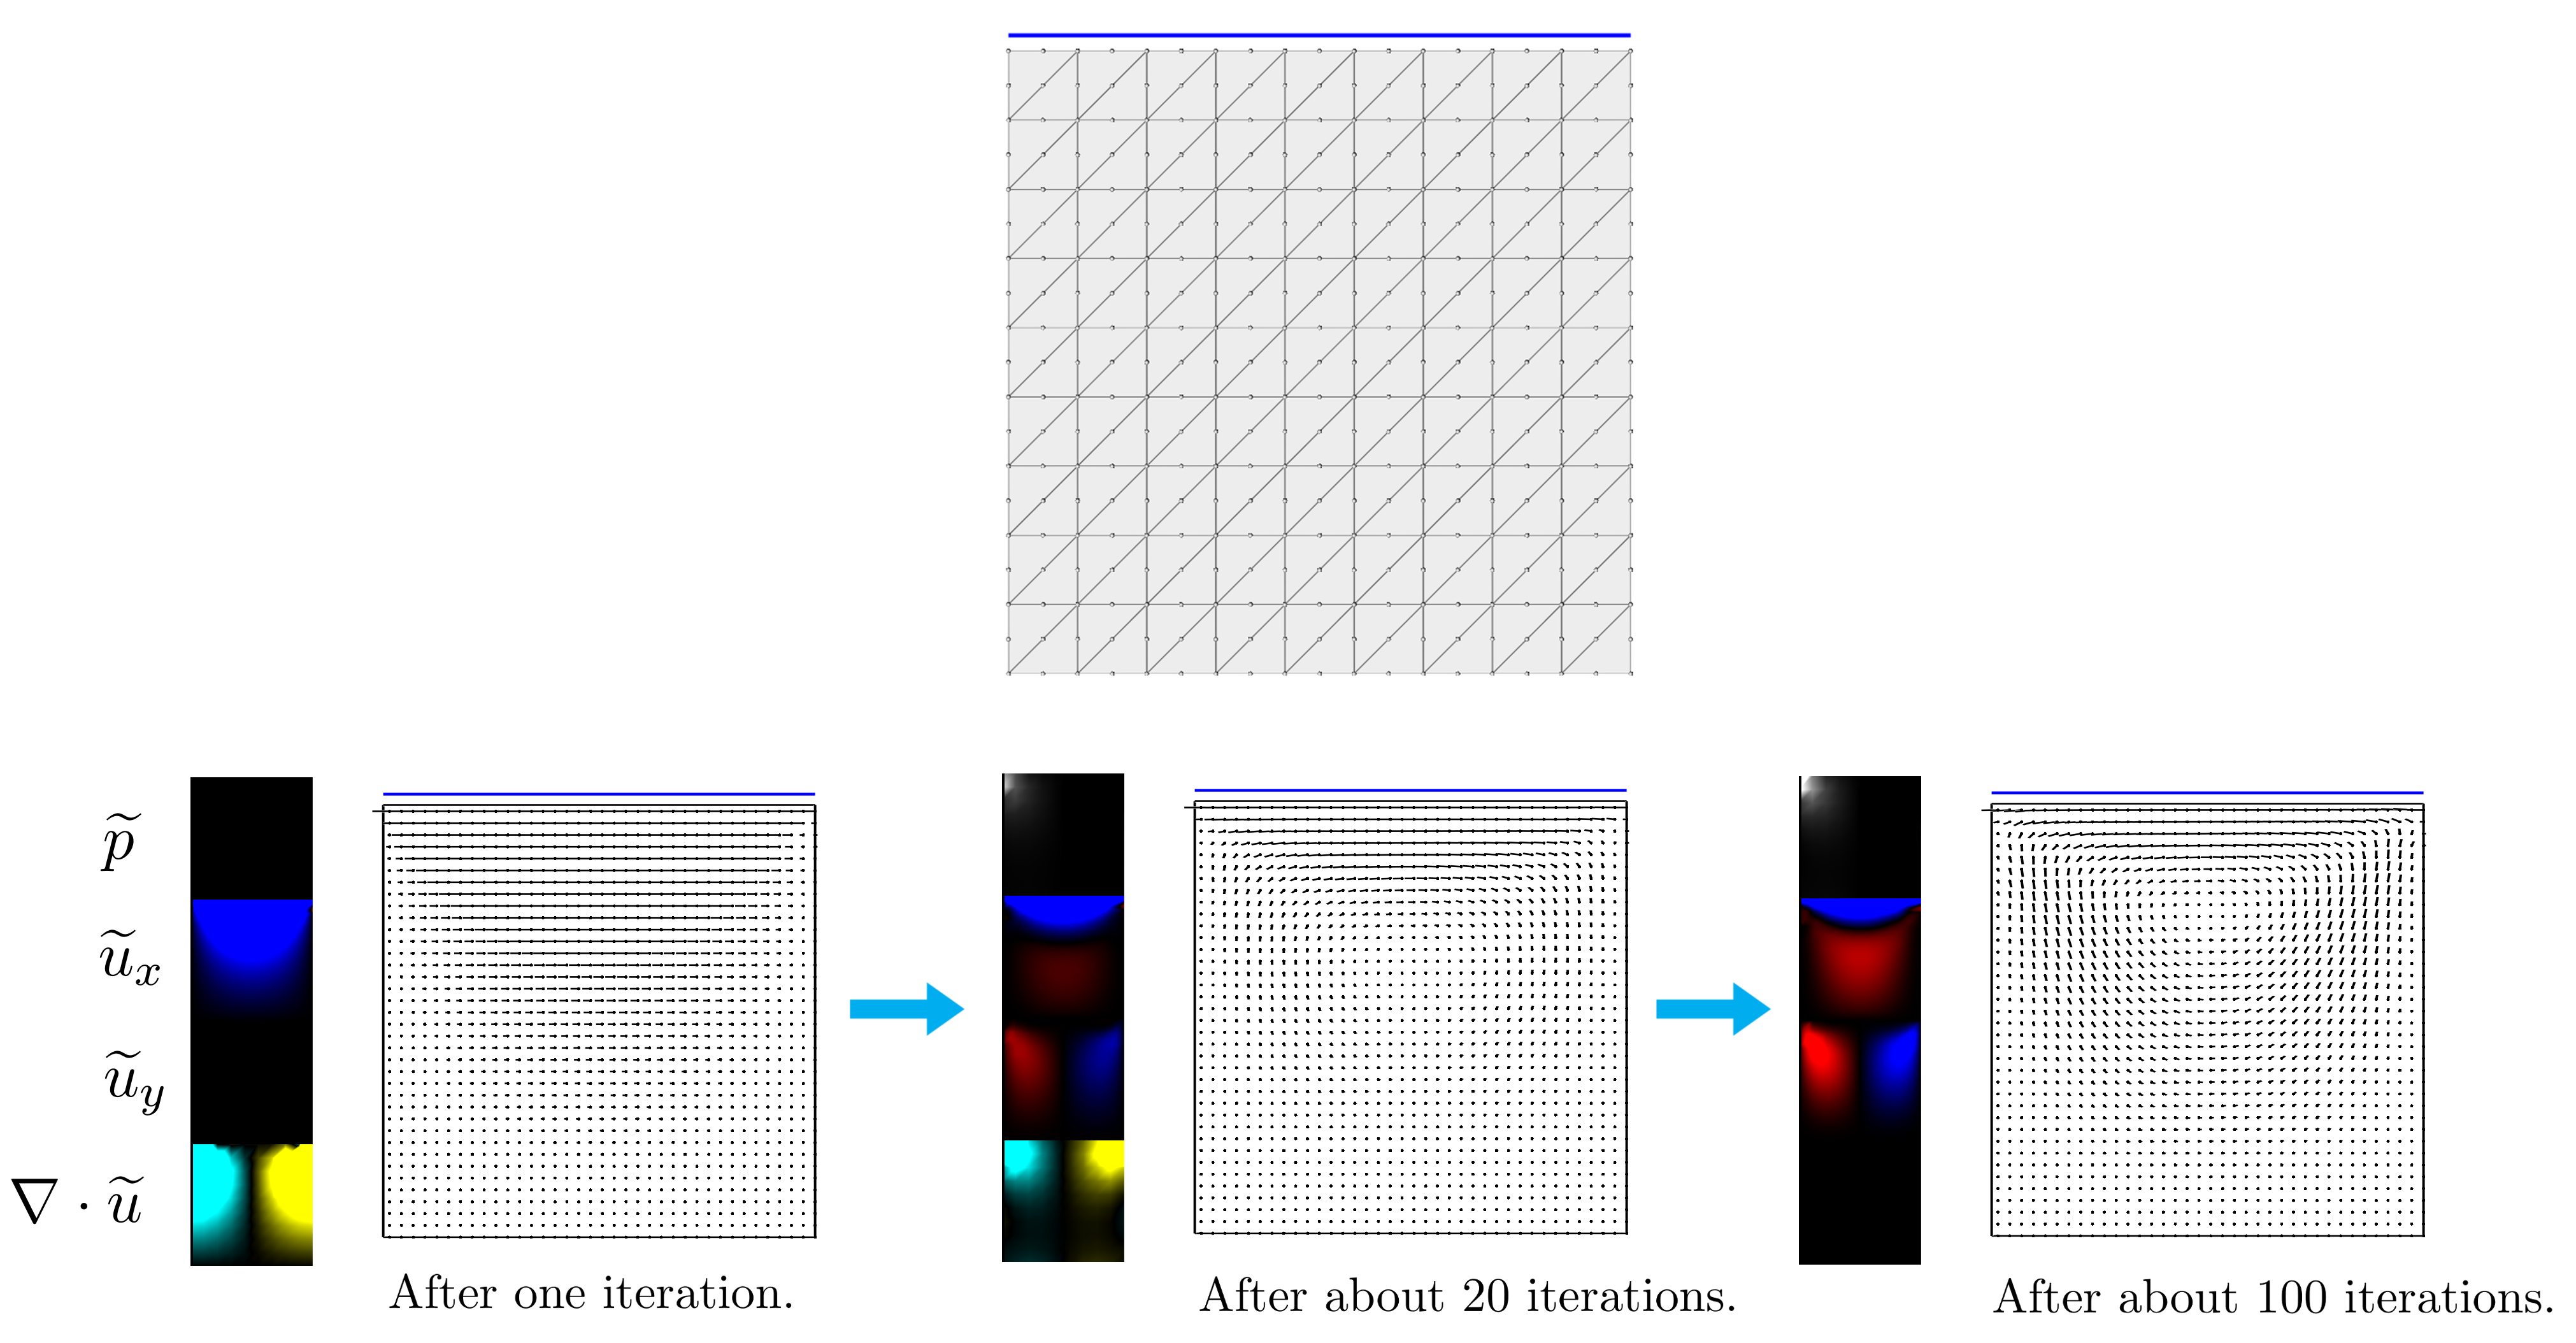
\includegraphics[width=1.1\textwidth]{figures/stokes/lid_driven_weakly_incompressible/figure.png}}
    \caption{\tiny
        The (scaled) velocity field is visualized by a regular grid of samples in the domain.
        The constraint residual $\nabla\cdot \widetilde{u}$ is displayed at the left, with cyan and yellow denoting opposite signs. The iterative pressure update
        progressively eliminates this residual.
    }
    \label{stokes_lid_driven_weakly_incomprssible}
\end{figure}

This has taken quite a large number of iterations, where two large sparse linear systems are solved each iteration (the Gramian system being the cheaper to solve).
The result is as expected, and this method is easy to implement given an already working quadratic-element Poisson solver.
However, as implemented, this method is neither general enough nor fast enough to form the basis of a Navier-Stokes solver.


% We will begin by discretizing the \textit{unconstrained} steady Stokes equations,
% which are a vector Poisson equation:
% \begin{equation}\label{steady_stokes_unconstrained}
%     -\mu\Delta u = \rho g.
% \end{equation}
% % >>>
% \subsection{Discretizing the vector Poisson equation}\label{discretizing_vector_poisson}
% % <<<
% In principle we should keep the Stokes equation
% in integral form (using the conservative-form Cauchy momentum equation \eqref{cauchy_continuity_eulerian}), and continue as we did
% in section \ref{trial_function}. However,
% we will take a formal step to skip the reasoning of section \ref{trial_function}, typical of finite element method derivations.
% As we start with the \textit{differential} equation \eqref{steady_stokes_unconstrained}, we can introduce a trial space $\Psi$ and then ``weaken''
% the equation by integrating against $v \in \Psi$, and removing the Laplacian by integration by parts:
% \begin{equation}\label{steady_stokes_unconstrained_weak}
%     \int_\Omega -\mu\Delta u\cdot v\,dx = \int_\Omega \rho g\cdot v\,dx
%     \quad\equiv\quad
%     \int_\Omega -\mu\nabla u : \nabla v\,dx = \int_\Omega \rho g\cdot v\,dx.
% \end{equation}

% Noting that the left-hand-side of \eqref{steady_stokes_unconstrained_weak} is a bilinear form in $u$ and $v$, and the right-hand-side
% is a linear functional in $\psi$, it is standard practice (ref) to write this kind of equation as
% \begin{equation}
%     a(u, v) = f(v).
% \end{equation}
% Our subsequent derivations are much the same as in \ref{discretizing_poisson}, simplified by our new notation.
% We can now approximate $u$ in the test space $\Phi$ as $\hat{u} = \sum_{i=1}^nu_i\phi_i$. By linearity we only need to compute
% trials over the basis trial functions $\psi_j$.
% We then have the linear system of equations
% \begin{equation}\label{elliptic_bilinear_form}
%     \sum_{i=1}^n u_i a\left(\phi_i, \psi_j\right) = f(\psi_j),\quad j=1,\cdots,n,
% \end{equation}
% which can be written in matrix form as
% \begin{equation}\label{elliptic_bilinear_form_matrix}
%     A\hat{u} = \begin{bmatrix}
%             a(\phi_1, \psi_1) & \cdots & a(\phi_1, \psi_n) \\
%             \vdots & & \vdots \\
%             a(\phi_n, \psi_1) & \cdots & a(\phi_n, \psi_n)
%             \end{bmatrix}
%     \begin{bmatrix} u_1 \\ u_2 \\ \vdots \\ u_{n-1} \\ u_n \end{bmatrix}
%     =
%     \begin{bmatrix} f(\psi_1) \\ f(\psi_2) \\ \vdots \\ f(\psi_{n-1}) \\ f(\psi_{n}) \end{bmatrix}
%     = \hat{f}.
% \end{equation}
% % The matrix $A$ is symmetric positive-definite, and we can therefore think of a solution to \eqref{elliptic_bilinear_form_matrix}
% % as as a minimizer of the scalar quadratic form
% % \begin{equation}\label{elliptic_quadratic_form}
% %     \hat{E}(\hat{u}) \coloneqq \frac{1}{2} \inner{\hat{u}, A\hat{u}} - \inner{\hat{u}, \hat{f}}.
% % \end{equation}
% % This is simply a discrete realisation of the fact that we can, as described in section \ref{pressure_derivation}, think
% % of a solution to the vector Poisson equation as a minimizer of the Dirichlet energy \eqref{steady_stokes_dirichlet_energy},
% % \begin{align*}
% %     E(u) \coloneqq \int_{\Omega} \frac{\mu}{2} \inner{\nabla u, \nabla u} - \rho g\cdot u \,dx.
% % \end{align*}
% We can solve \eqref{elliptic_bilinear_form_matrix} to get a velocity field $\sum_{i=1}^n u_i\phi_i$, although in general this will not satisfy $\nabla\cdot u = 0$.
% As some preliminary analysis, if $\Phi = \Psi$ and have the same basis functions, we have a symmetric-positive-definite system. This form of linear system is known to be stably solvable,
% for example by the conjugate gradient method.
% >>>

\section{A mixed finite element method}
As described in section \ref{pressure_derivation}, the pressure $p$ is a Lagrange multiplier that appears
when solving the optimization problem \eqref{stokes_flow_optimization}:
\begin{equation*}
\begin{aligned}
& \underset{u}{\text{minimize}}
& & E(u) =  \frac{\nu}{2} \inner{\nabla u, \nabla u} - \inner{u, \rho g}\\
& \text{subject to}
& & \nabla\cdot u = 0.
\end{aligned}
\end{equation*}

\newcommand{\trialconstraint}{{\Psi_{\text{constraint}}}}
\newcommand{\testpressure}{{\Phi_{\text{pressure}}}}
It is natural, then, to introduce $p$ as a variable to solve for. Solving for the pressure (the ``dual variable'') simultaneously with the velocity
(the ``primal variable'')
is called a primal-dual method for the optimization \eqref{stokes_flow_optimization}, and the resulting finite element method is called \textit{mixed}.

\subsubsection{The pressure finite element space}
Pressure then needs to be discretized, so we introduce another test space $\Phi^p$.
To get a weak form of the steady Stokes equations \eqref{steady_stokes}, including the constraint $-\nabla\cdot u = 0$
(where the negative sign is introduced in order to introduce some structure to the resulting linear system, apparent later), we introduce
another trial space $\Psi^p$, whose functions will be integrated against $-\nabla\cdot u$.

\subsubsection{The velocity finite element product space }
Further, we introduce a $2n_u$--dimensional vector finite element space for velocity as a product of scalar finite element spaces
\footnote{
There are other ways to create finite element spaces of vector fields, which are not equivalent to product spaces of scalar finite element spaces,
but this is the simplest choice.}:
$$
    \Phi^u = \Phi^{u,s} \times \Phi^{u,s}.
$$
A natural choice for the basis functions of $\Phi^u$ is:
\begin{equation}\label{velocity_product_basis}
\Phi^u = \text{span}\left\{\phi_1^{u,s}\partial x, \phi_1^{u,s}\partial y,
    \cdots,
    \phi_{n_u}^{u,s}\partial x, \phi_{n_u}^{u,s}\partial y
\right\},
\end{equation}
where $\partial x$ and $\partial y$ denote unit vector fields in the axis directions.

\subsection{The mixed weak form of the steady Stokes equations}
The weak form of the steady Stokes equations \eqref{steady_stokes} is then
\begin{equation*}
\begin{split}
    &\int_\om \left(-\nu\Delta u + \nabla p\right)\cdot \psi^u\,d\hat{x} = \int_\Omega \rho g\cdot\psi^u\,d\hat{x},\\
    &\int_\om -\psi^p\left(\nabla\cdot u\right)\,d\hat{x} = 0, \quad\text{for all $\psi^u \in \Psi^u, \psi^p \in \Psi^p$},
\end{split}
\end{equation*}
which by integration by parts can be written as
\begin{equation}\label{steady_stokes_weak}
\begin{split}
    &\int_\om \nu\nabla u : \nabla \psi^u - p\nabla\cdot \psi^u\,d\hat{x} = \int_\om \rho g \cdot \psi^u\,d\hat{x},\\
    &\int_\om -\psi^p\left(\nabla\cdot u\right)\,d\hat{x} = 0, \quad\text{for all $\psi^u \in \Psi^u, \psi^p \in \Psi^p$},
\end{split}
\end{equation}
This can be thought of as a single set of equations integrated against basis functions in the ``mixed'' finite element spaces
    $$\Phi^\mathcal{M} = \Phi^u \oplus \Phi^p \text{\quad and \quad} \Psi^\mathcal{M} = \Psi^u \oplus \Psi^p$$
where $\Phi^\mathcal{M}$ has basis functions
\begin{equation}\label{mixed_space_basis_functions}
    \Phi^\mathcal{M} = \text{span}\left\{
        \phi^u_1,\cdots,\phi^u_{2n_u}, \phi_1^p,\cdots,\phi_{n_p}^p
    \right\}
\end{equation}
and similar for $\Psi^\mathcal{M}$.
The sum of a velocity basis function $\psi^u$ with a pressure basis function $\psi^p$ is a formal sum $\psi^u + \psi^p$. The weak form is then
\begin{equation}\label{steady_stokes_weak_mixed}
\begin{split}
    &\int_\om \nu\nabla u : \nabla \psi^u - p\nabla\cdot \psi^u
    -\psi^p\left(\nabla\cdot u\right)\,d\hat{x}
 = \int_\om \rho g \cdot \psi^u\,d\hat{x},\\
    &\text{for all $\psi^u + \psi^p \in \Psi^\mathcal{M}$}.
\end{split}
\end{equation}
We will not use this formalism, but it is helpful when automating the finite element method \cite{automating_fem}.
This mixed space (with a P2 product space for velocity and a P1 space for pressure), forms the ``Taylor-Hood elements'', and is known to result in a stable method for the Stokes problem \footnote{
While we could choose just about any spaces for the non-mixed method for the Poisson problem, which gives a symmetric positive-definite 
system when $\Phi = \Psi$, the Stokes flow problem
inherently involves a Lagrange multiplier, and is known as a ``saddle point problem''. The resulting finite element matrix is symmetric mixed-definite.
The Taylor-Hood elements satisfy the Ladyzhenskaya--Babu\v ska--Brezzi (LBB) condition, which
is a theoretical result which guarantees that the resulting linear system for the Stokes problem will be well-conditioned.
If we took velocity to be in $P_1 \times P_1$ instead, for example, this condition would not hold.
}.

% So we don't have to repeat the equations for each kind of mixed trial function, as we do in \eqref{stokes_flow_mixed_equations_1}, we can use the mixed basis order \eqref{mixed_space_basis_functions} and define $\phi^\mathcal{M}_l$ to be the $l$'th mixed basis
% function in this order (e.g. $\psi^\mathcal{M}_1 = (\psi_1, 0)$ and $\psi^\mathcal{M}_{n+1} = (0, \psi^p_1)$).
% 
% \begin{aside}
% \textit{A note on tensor notation for the vector field space}
% \vskip 0.1in
% 
% The space $P^2_2$ here is a space of piecewise quadratic vector fields formed as $P^2_2 = P^2 \times P^2$.
% This represents the velocity field by two functions in the usual scalar quadratic space $P^2$.
% This is the simplest way to construct a finite element space of vector fields, although others (not based on a product construction) are possible.
% We define $\partial x$ and $\partial y$ to be the unit vector fields on the domain $\Omega$.
% The basis functions for $P^2_2$ are the natural choice of vector fields $\phi^\text{scalar}_1\partial x$, $\phi^\text{scalar}_1\partial y$, $\cdots$, $\phi^\text{scalar}_n\partial x$, $\phi^\text{scalar}_n\partial y$.
% However, we would like to think of the velocity coefficients as vector samples, rather than scalar coefficients
% of this array of $2n$ basis vector fields. We can do this by letting $\phi_1,\cdots,\phi_n$ be aggregates of axis-aligned vector fields:
%     $$
%         \phi_i = \begin{bmatrix}
%         \phi_{ix} \coloneqq \phi^\text{scalar}_{i}\partial x\\
%         \phi_{iy} \coloneqq \phi^\text{scalar}_{i}\partial y\end{bmatrix}.
%     $$
% We can then represent the interior variation as
%     $$\tilde{u}_\text{interior} = \sum_{i=1}^n u_i \cdot \phi_i.$$
% It is important to keep this in mind, as although this notation is natural, it may cause confusion:
% While $a$ is a bilinear form, the value $a((\phi_1, 0), \psi^\mathcal{M}_4)$, for example, is actually ``vectorized''
% into
%     $$
%         \begin{bmatrix}
%             a((\phi_{1x}, 0), \psi^\mathcal{M}_4)\\
%             a((\phi_{1y}, 0), \psi^\mathcal{M}_4)
%         \end{bmatrix}.
%     $$
% This is contracted with the vector coefficient $u^1$ to get a scalar:
%     $$
%         u^1 \cdot a((\phi_1, 0), \psi^\mathcal{M}_4)
%     = u^1_x a((\phi_{1x},0), \psi^\mathcal{M}_4)
%         + u^1_y a((\phi_{1y},0), \psi^\mathcal{M}_4).
%     $$
% \end{aside}

\subsection{Forming a linear system from the mixed weak form}
Let $u$ be approximated by
$$\tilde{u} = \tilde{u}_\Gamma + \tilde{u}_\text{interior} = \tilde{u}_\Gamma +
    \sum_{i=1}^{n_u}\left[
    u_{xi}\phi^{u,s}_i\partial x
    +
    u_{yi}\phi^{u,s}_i\partial y\right],
$$
where $\tilde{u}_\Gamma \in \Phi^{*,u}$ approximates the Dirichlet boundary function $\left.u\right|_\Gamma = u_\Gamma$,
and $\tilde{u}_{\text{interior}} \in \Phi^u$ is the ``interior variation''.
$\Phi^{*,u}$ is the full P2 vector finite element space, which is not required to be zero on the boundary.
A boundary condition for pressure is not given. Pressure is approximated as
    $$\tilde{p} = \sum_{i=1}^{n_{p-1}} p_i\phi^p_i.$$
The last pressure node, $p_n$, is fixed at $p_n = 0$, so that a unique pressure is determined up to some arbitrary constant.
Now, substituting $u \leftarrow \tilde{u}$ and $p \leftarrow \tilde{p}$, the mixed weak form \eqref{steady_stokes_weak} expands to
\begin{equation}\label{steady_stokes_linear_system}
\begin{split}
&\sum_{i=1}^{n_u} \left[u_{xi}\int_\Omega \nu\nabla\phi^{u,s}_i \cdot \nabla\psi^{u,s}_j\,d\hat{x}\right]
        + \sum_{i=1}^{n_p} p_i\int_\Omega -\psi^{u,s}_j \Part{\phi^p_{i}}{x}\,d\hat{x}
    = \int_\Omega \rho g_x \psi^{u,s}_j
        - \nu\nabla\widetilde{u}_{\Gamma,x} \cdot \nabla\psi^{u,s}_j \,d\hat{x},\\
    &\sum_{i=1}^{n_u} \left[u_{yi}\int_\Omega \nu\nabla\phi^{u,s}_i \cdot \nabla\psi^{u,s}_j\,d\hat{y}\right]
            + \sum_{i=1}^{n_p} p_i\int_{\Omega} -\psi^{u,s}_j \Part{\phi^p_{i}}{y}\,d\hat{x}
        = \int_\Omega \rho g_y \psi^{u,s}_j
            - \nu\nabla\widetilde{u}_{\Gamma,y} \cdot \nabla\psi^{u,s}_j \,d\hat{x}\\
    &\text{for \quad} j=1,\cdots,n_u,\\
    &\sum_{i=1}^{n_u} \left[u_{ix} \int_\Omega -\psi^p_j \Part{\phi^u_i}{x} \,d\hat{x}
    + u_{iy} \int_\Omega -\psi^p_j \Part{\phi^u_i}{y} \,d\hat{x}\right]
        = \int_\Omega \psi^p_j \nabla \cdot \widetilde{u}_\Gamma\\
    &\text{for \quad} j=1,\cdots,n_p-1.\\
\end{split}
\end{equation}
The duplication of the terms of this equation is due to the product-space nature of $\Phi^u$. The $\phi^u$ and $\psi^u$ terms
in the weak form have been replaced by the velocity product-space basis functions \eqref{velocity_product_basis}, resulting
in some partial derivatives rather than divergences. The result is a $(2n_u + n_p - 1)\times (2n_u + n_p - 1)$ linear system.


\subsection{Implementation and results}
As each basis function has a small support, the resulting linear system will be highly sparse, and, as in chapter 3, each integral coefficient, bar
those involving the
the source term $\rho g$, can be computed analytically by changes of variables onto reference triangles. The resulting tables of ``magic numbers'',
and implementations of mesh traversals to form these matrix coefficients, is a somewhat tedious and routine task, but forms the core of complexity
in the implementation of this method --- and is a good target for automation \cite{automating_fem} \cite{fenics_book} \cite{firedrake}. For this matrix to be constructed efficiently, as described in chapter 3, a good mesh data structure is necessary
for fast mesh traversal to find overlapping basis functions. The bottleneck of this algorithm is then the solution of the resulting
large, sparse, symmetric mixed-definite system.

I have implemented this method in C\texttt{++} using the same mesh data structure and linear algebra library (Eigen3 \cite{eigen})
used to implement the Poisson equation solvers in chapter 3.

\subsubsection{Lid driven cavity with obstruction}
The results for the lid-driven cavity problem, with $\nu = 1$, and an additional complex obstruction, are displayed in figure
\ref{stokes_lid_driven_obstruction}.
The colour maps display a scaled pressure (white denoting high pressure), the velocity components
(with blue denoting a negative value, red a positive value), and the divergence projected into P1.
The incompressibility condition does in fact
hold to within a small margin of error on the order of $10^{-4}$.

% \begin{equation}
% \begin{split}
%     \sum_{i=1}^{n_u}\left[
%         u_{ix}\int_\Omega\mu\nabla\phi_{ix}^u:\nabla\psi_j^u\,d\hat{x}
%         +
%         u_{iy}\int_\Omega\mu\nabla\phi_{iy}^u:\nabla\psi_j^u\,d\hat{x}
%     \right]
%     +
%     \sum_{i=1}^{n_p} p_i\int_\Omega \phi_i^p\nabla\cdot\psi^u_j\,d\hat{x}
%     =
%     \int_\Omega\nabla\tilde{u}_\Gamma:\nabla\psi_j^u\,d\hat{x},\\
%     \text{\quad for $j=1,\cdots,2n_u$}.\\
%     \sum_{i=1}^{n_u}\left[
%         u_{ix}\int_\Omega\psi_k^p\nabla\cdot\phi_{ix}^u\,d\hat{x}
%         +
%         u_{iy}\int_\Omega\psi_k^p\nabla\cdot\phi_{iy}^u\,d\hat{x}
%     \right]
%     =
%     \int_\Omega\psi_k^p\nabla\cdot\tilde{u}_\Gamma\,d\hat{x},\\
%     \text{\quad for $k=1,\cdots,n_p$}.\\
% \end{split}
% \end{equation}

\begin{figure}[H]
    \centering
    \centerline{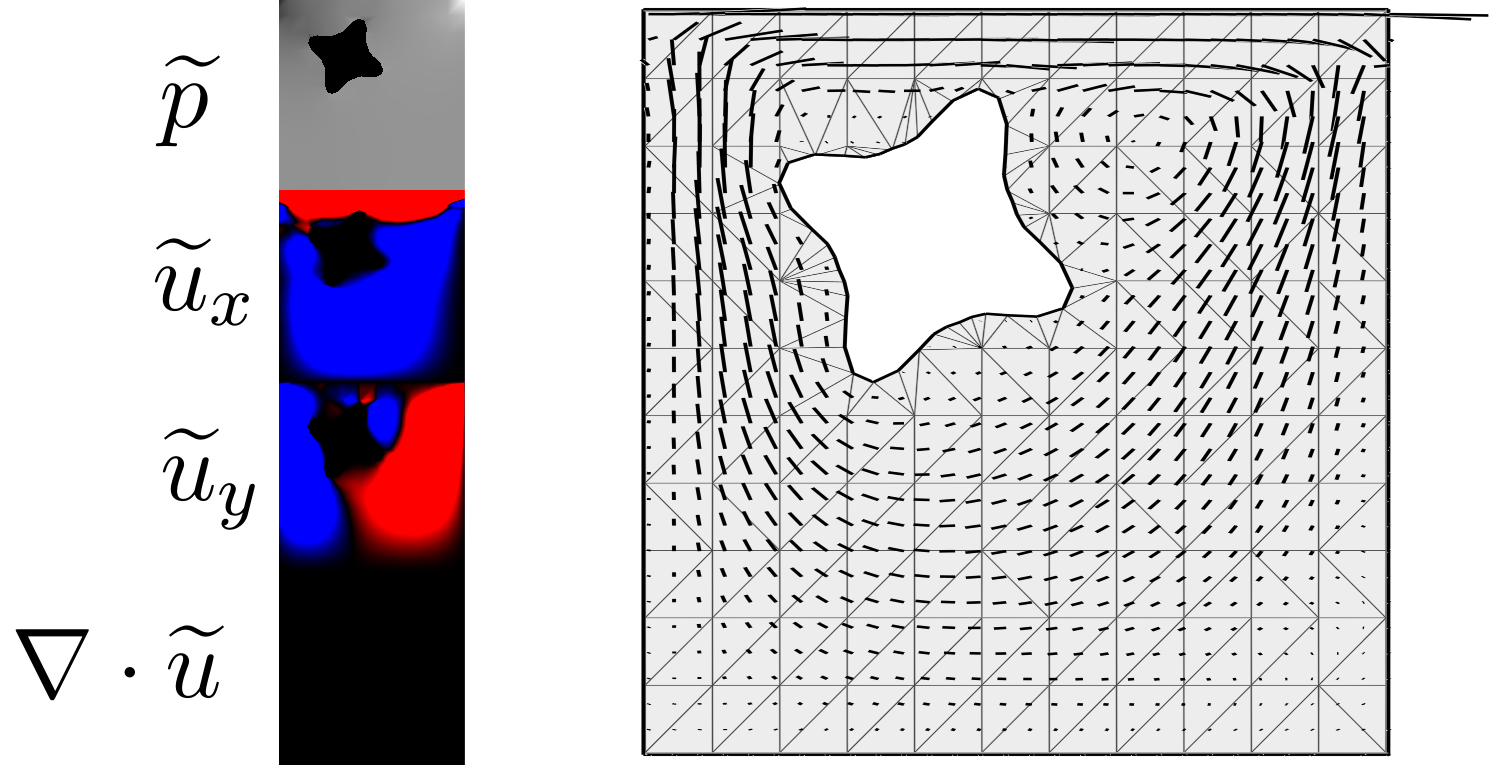
\includegraphics[width=0.7\textwidth]{figures/stokes/lid_driven_obstruction/figure.png}}
    \caption{\tiny
        The Stokes flow results for the lid-driven cavity problem, with kinematic viscosity $\nu = 1$.
        The additional obstruction causes the large vortex, created by the ``sliding lid'', to split.
    }
    \label{stokes_lid_driven_obstruction}
\end{figure}
\newpage
\subsubsection{Stokes flow around an obstruction in a pipe}
As an alternative test case, Stokes flow around an obstruction in a pipe can be simulated by making the pipe domain long enough.
The no-slip condition is enforced on
the two walls of the pipe, and Dirichlet conditions are given to emulate a constant flow from right to left. As the steady Stokes equations
are a constrained vector Poisson equation, \textit{any} Dirichlet condition will give a well-formed system, which is not necessarily true
if we instead enforce Neumann (boundary flux) conditions.
The results, and a basic overview of the process of this method, are shown in figure \ref{stokes_pipe}.
The linear system (with sparsity patterns for the matrix and right-hand-side vector, and the block matrix structure indicated by colour) is also visualised.
\begin{figure}[H]
    % \vskip -1in
    \centering
    \centerline{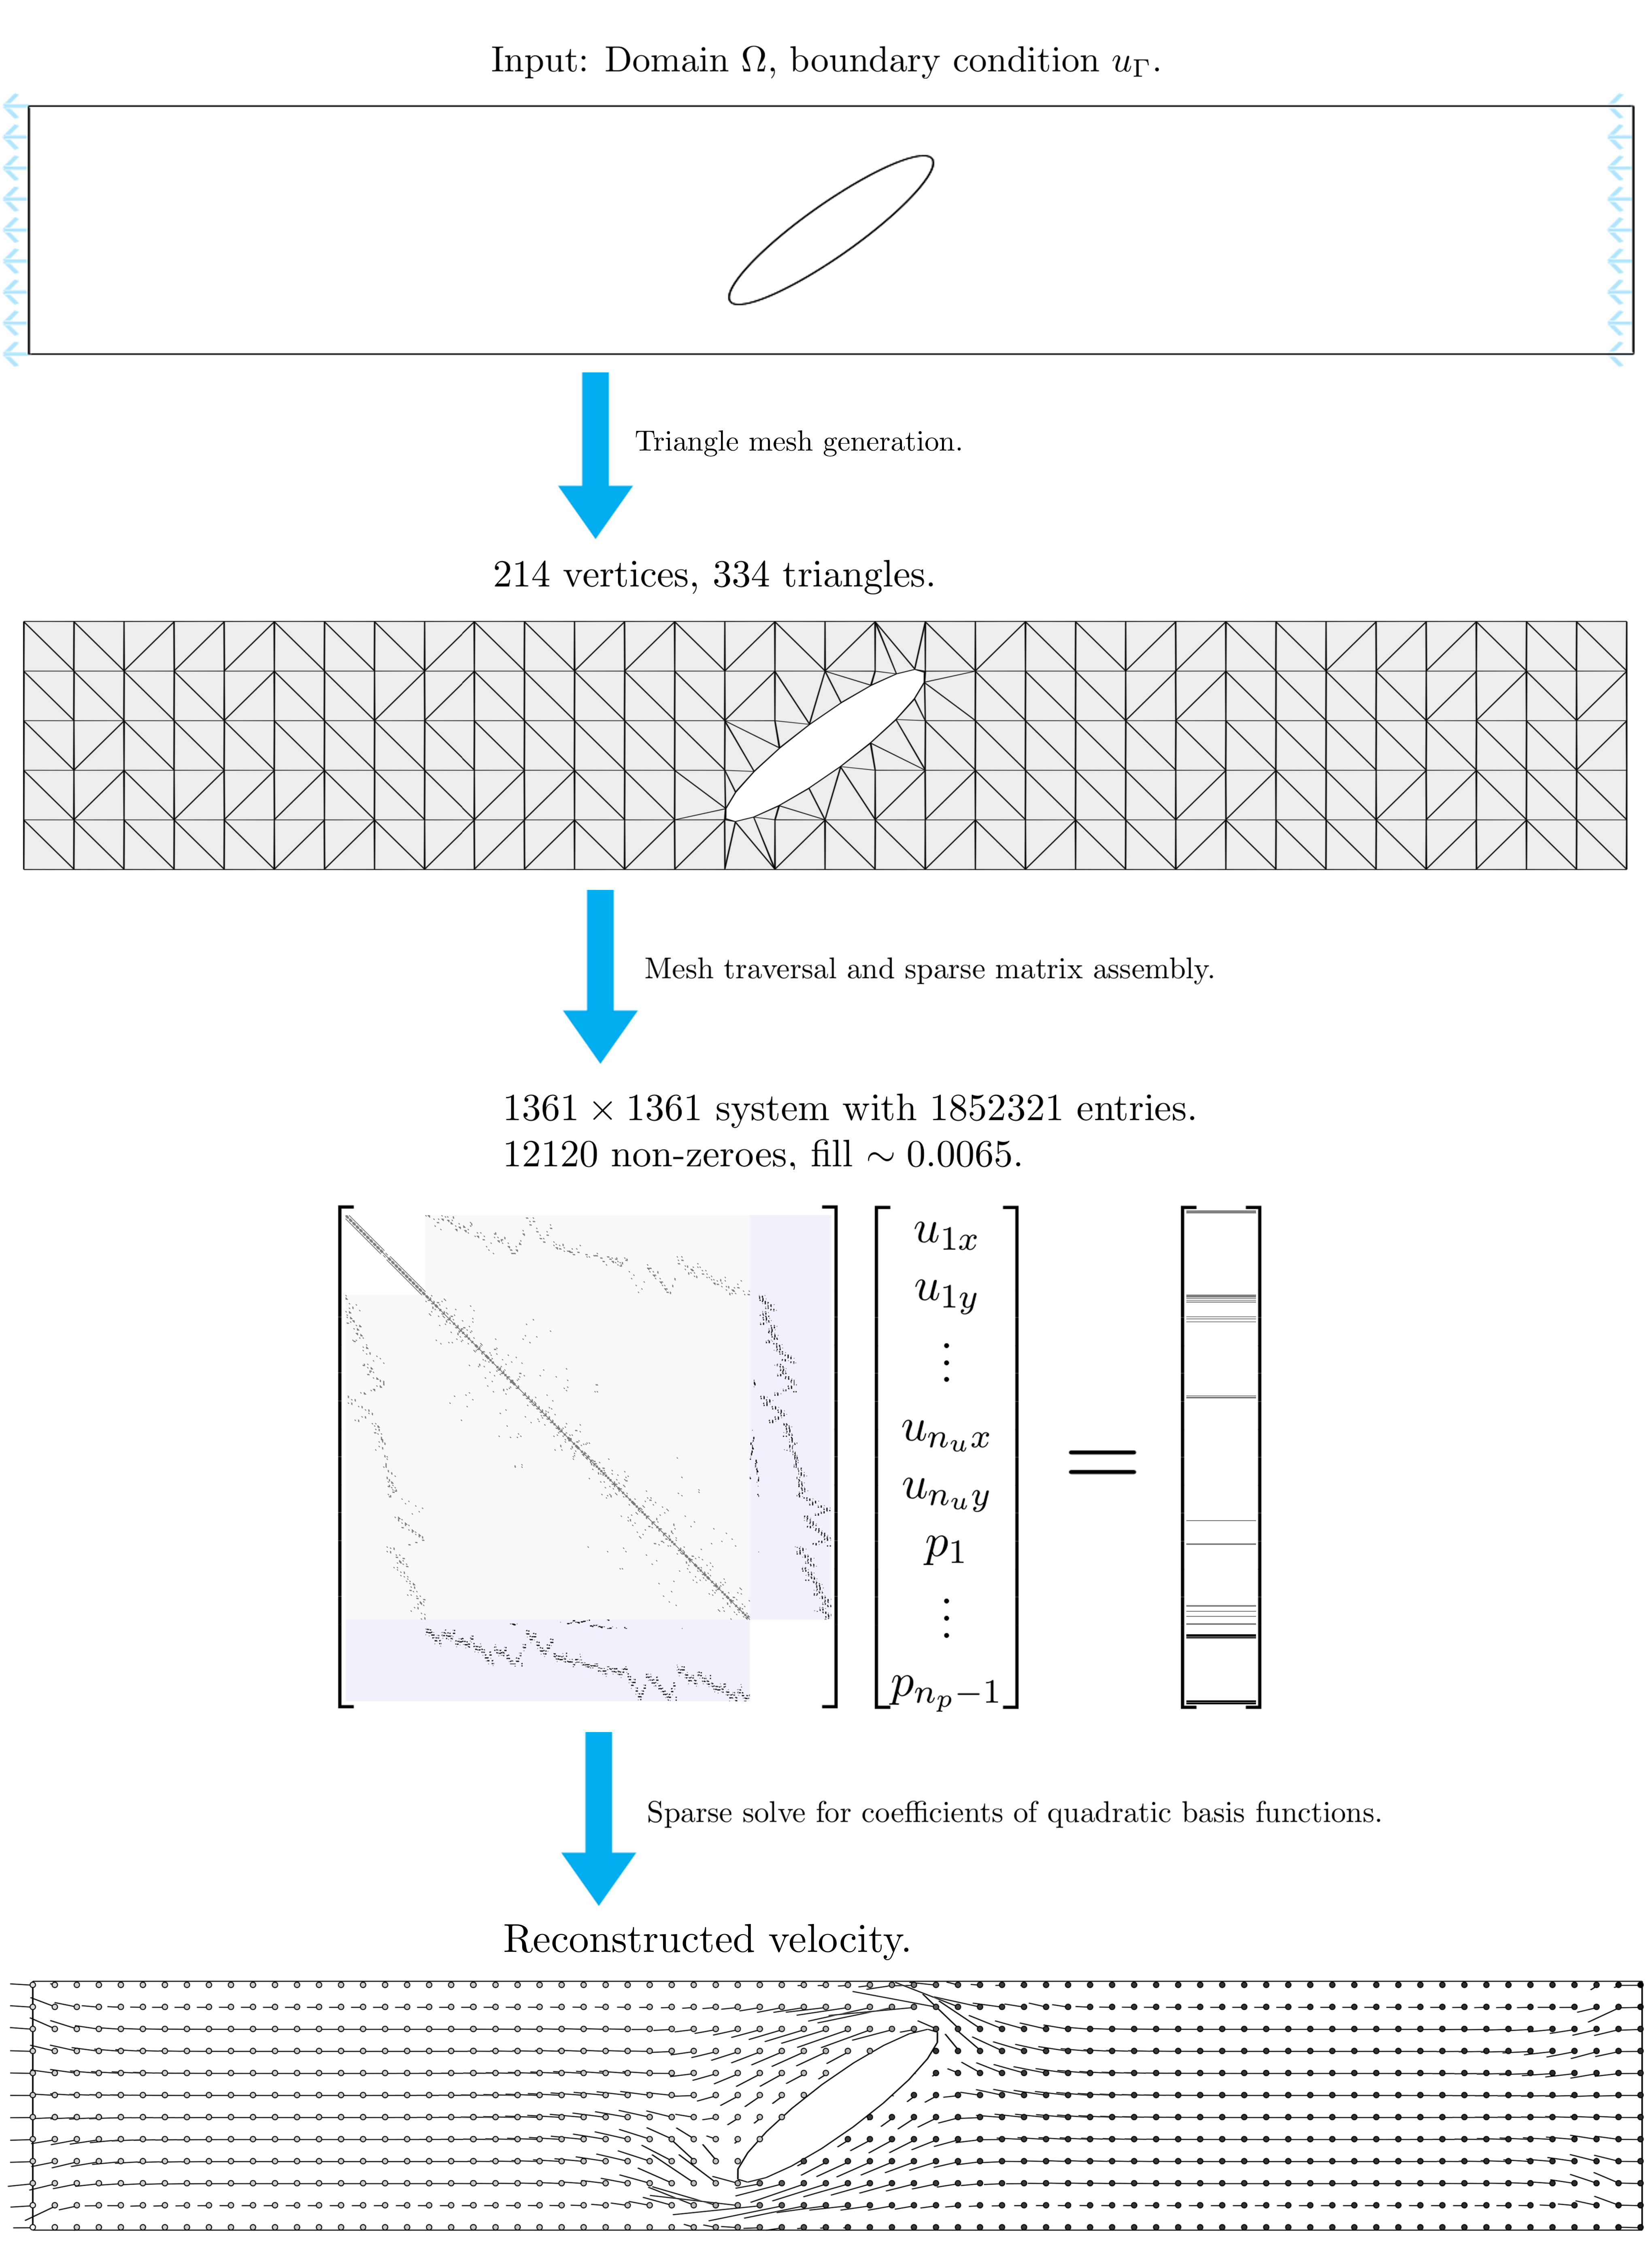
\includegraphics[width=0.9\textwidth]{figures/stokes/pipe/full.png}}
    \caption{The resulting finite element process for Stokes flow.
        % The finite element modelling process is visualised here for the particular case of Stokes flow through
        % a (shortened) long pipe around an obstruction. The algorithm consists of the construction of a large
        % sparse linear system on a generated mesh, which is then solved for the velocity and pressure. The velocity and pressure
        % are then reconstructed from the P2 and P1 basis functions.
    }
    \label{stokes_pipe}
\end{figure}

% The results are shown in figure \ref{stokes_pipe}.
% The linear system (with sparsity patterns and block matrix indicators the matrix and right-hand-side vector) is visualised in figure
% \ref{stokes_system}.
% \begin{figure}[H]
%     \centering
%     \centerline{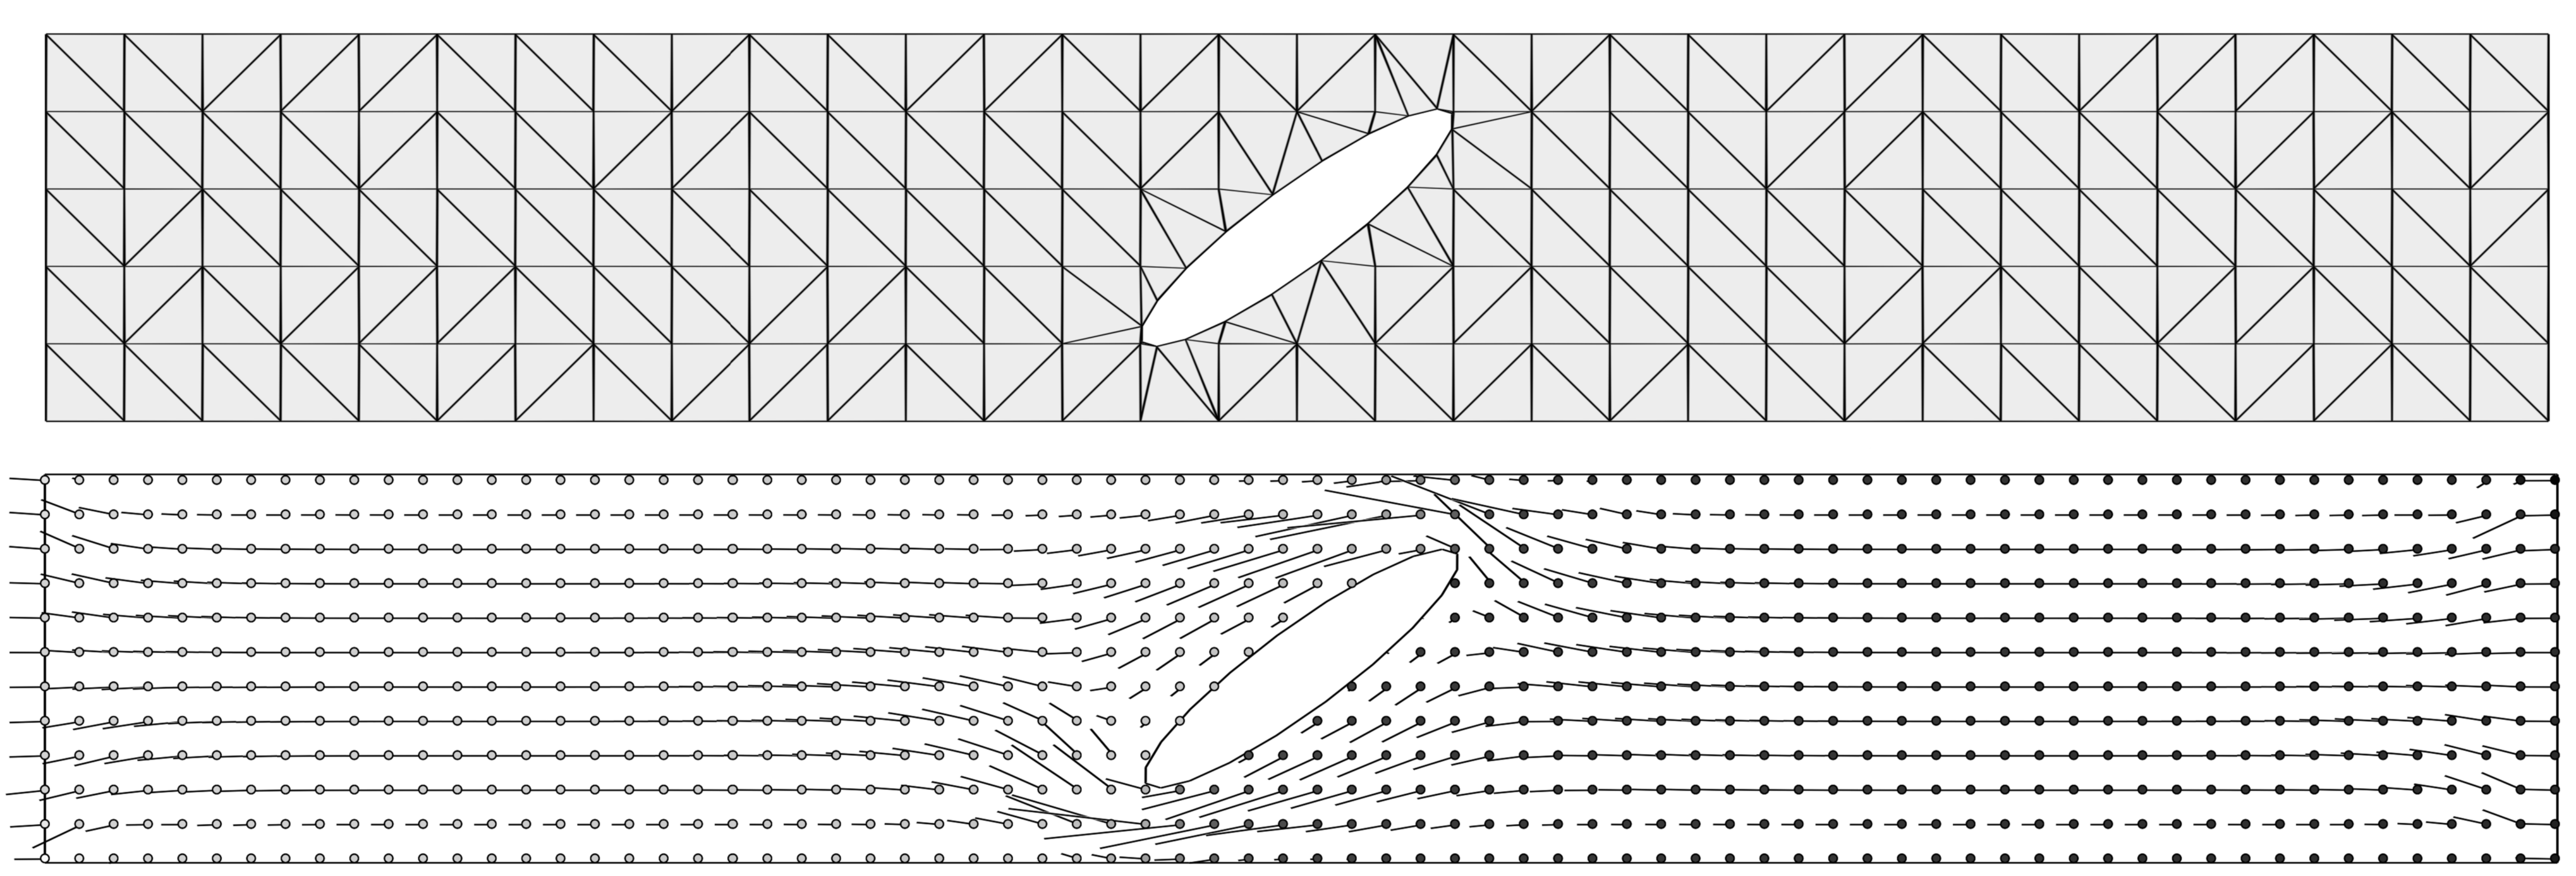
\includegraphics[width=1.3\textwidth]{figures/stokes/pipe/figure.png}}
%     \label{stokes_pipe}
% \end{figure}
% \begin{figure}[H]
%     \centering
%     \centerline{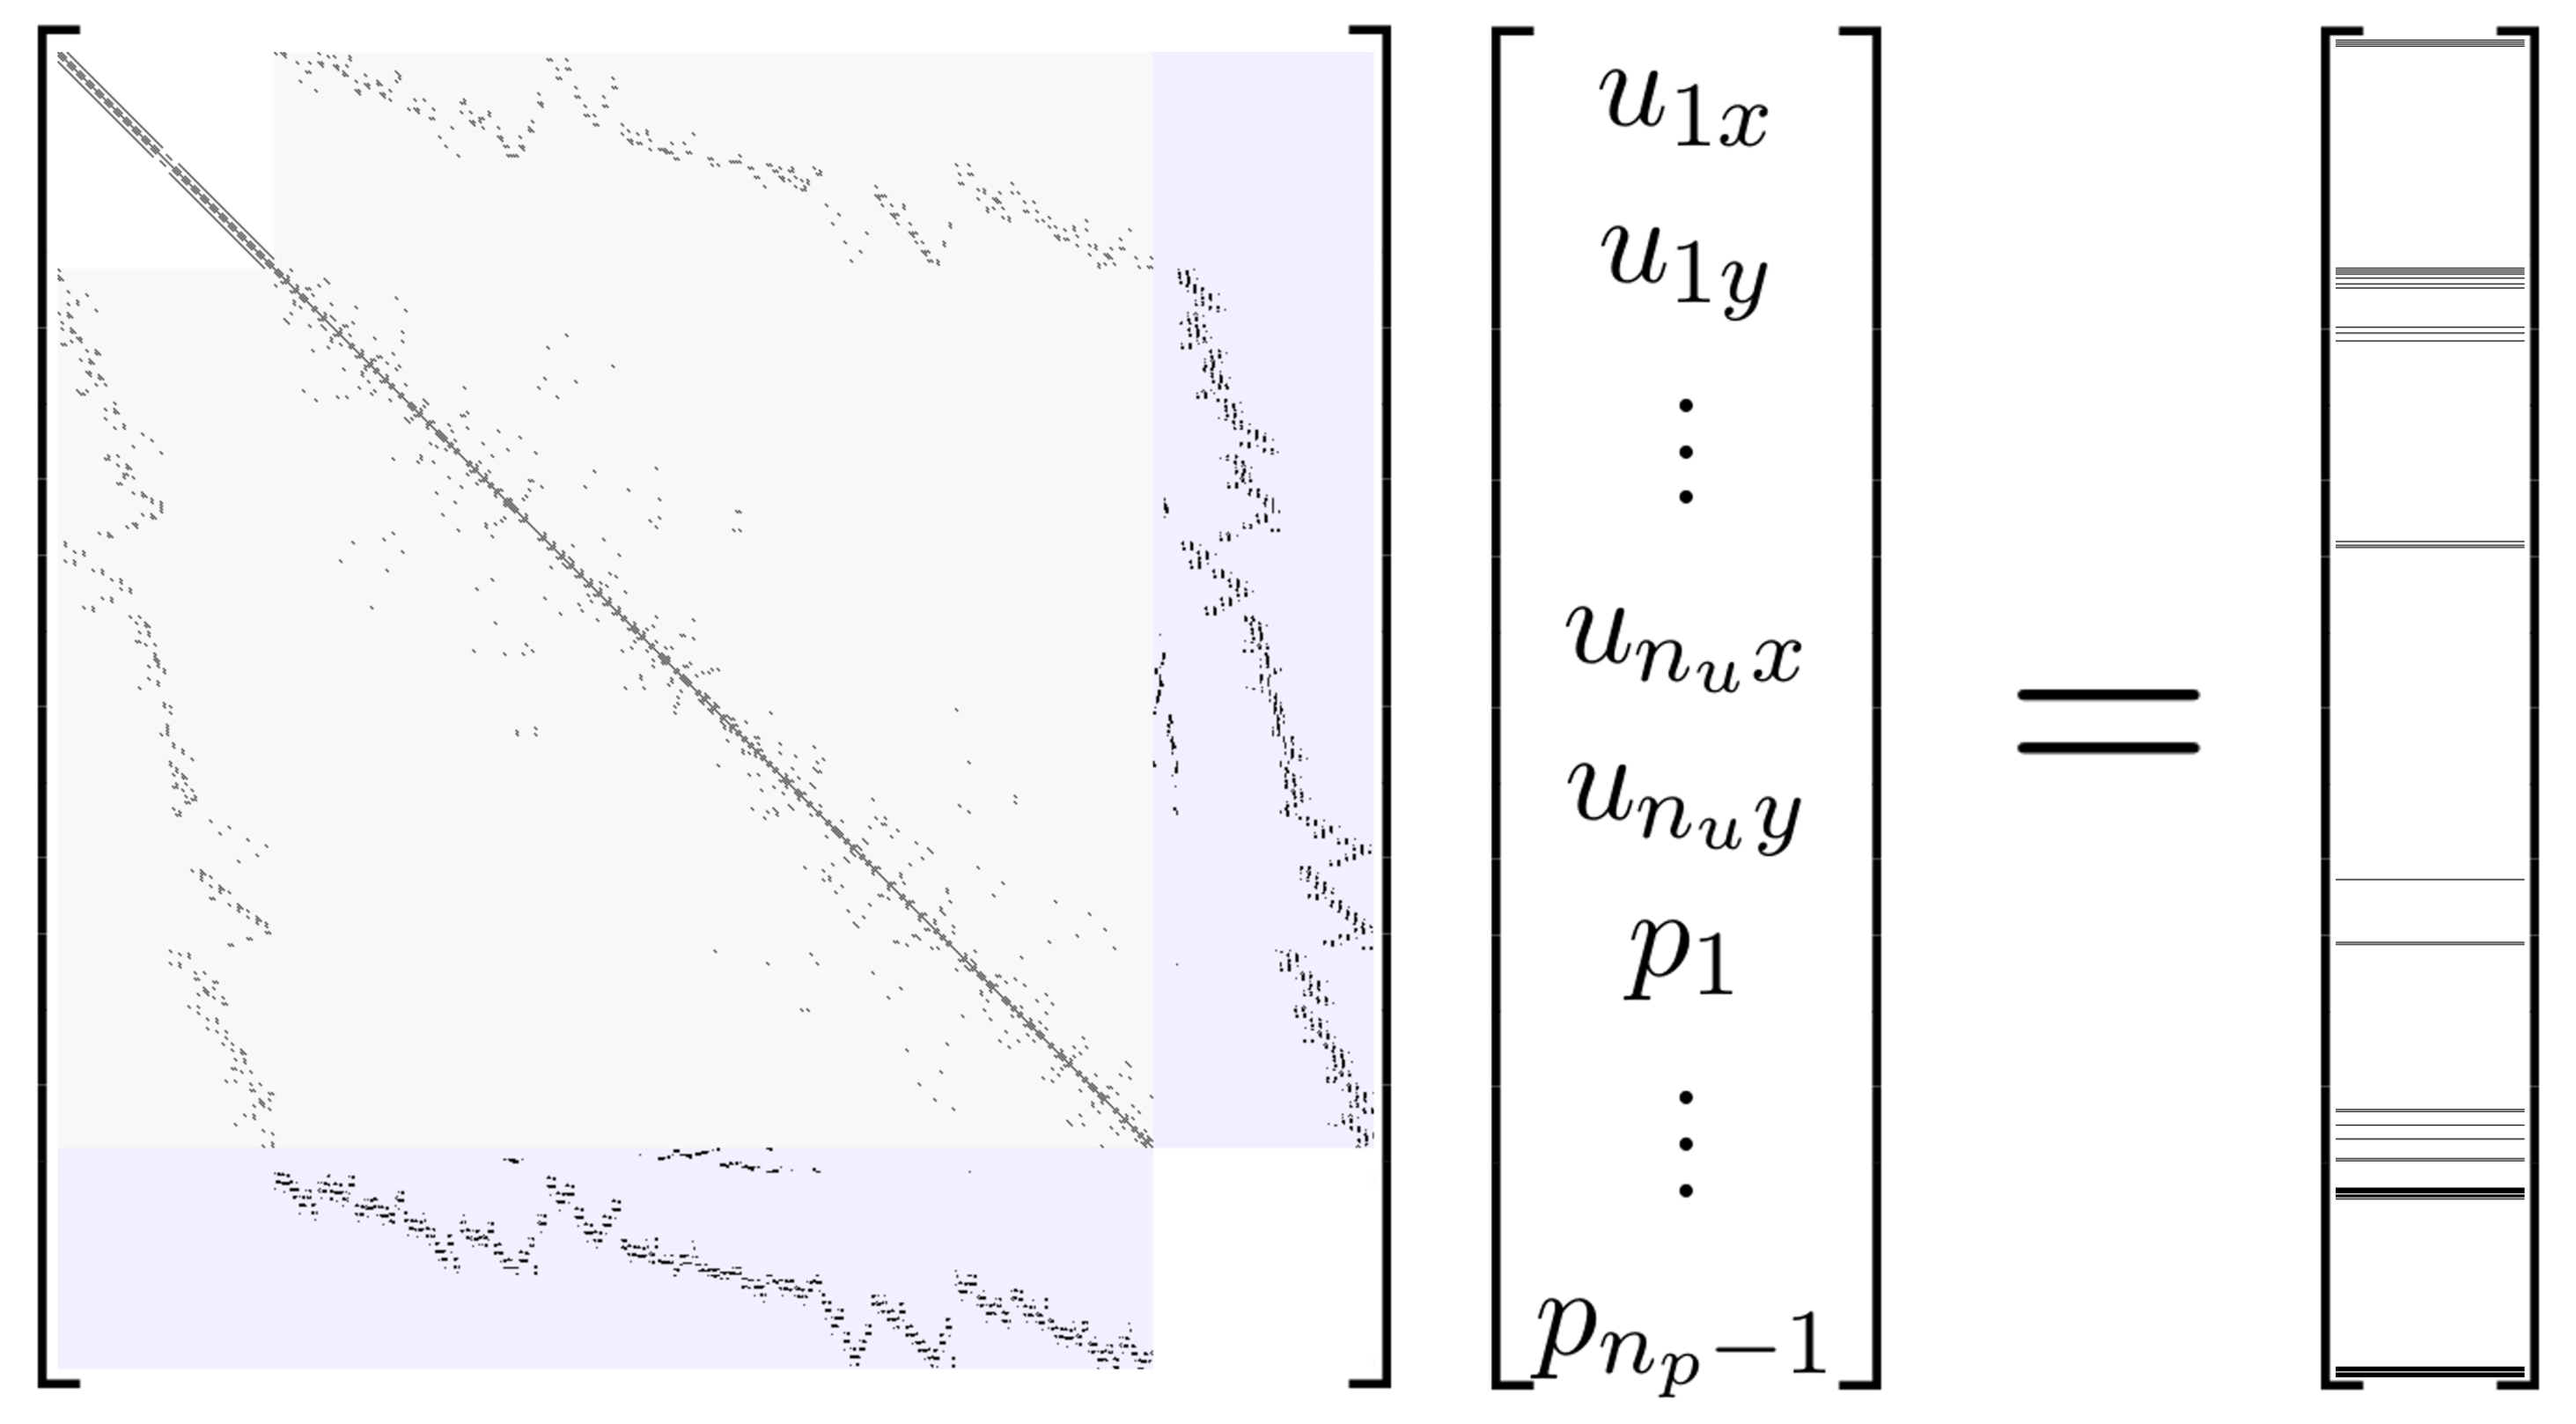
\includegraphics[width=0.7\textwidth]{figures/stokes/pipe/system.png}}
%     \label{stokes_system}
% \end{figure}



% \begin{align*}
%     &\widetilde{u}_x\\
%     &\widetilde{u}_y\\
%     &\widetilde{p}\\
%     &\nabla\cdot \widetilde{u}
% \end{align*}
% 
% After one iteration.
% 
% After about 20 iterations.
% 
% After about 100 iterations.
